This layer is the destination of all the instructions from the Control Layer go to. It contains the UR5's arm, its control box, and a Polyscope for the UI.

\subsection{UR5 Layer Hardware}
The UR5 is a sophisticated robot system developed and created by Universal Robotics. It contains a 6-jointed robotic arm that sends and receives data to control box. The control box itself sends and receives commands through the Polyscope, a large hand-held touch pad device.

\subsection{UR5 Layer Operating System}
N/A

\subsection{UR5 Layer Software Dependencies}
N/A

\subsection{UR5 Arm}
This subsystem consists of a 6-jointed arm that houses a servo for each of those joints that can rotate 360 degrees in either direction.  It receives signals from the control box to determine what pose should be in.

\begin{figure}[h!]
	\centering
 	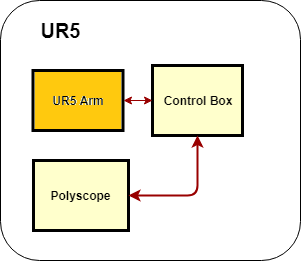
\includegraphics[width=0.60\textwidth]{images/UR5_Layer_UR5_Arm}
 \caption{UR5 Arm subsystem diagram}
\end{figure}

\subsubsection{UR5 Arm Subsystem Hardware}
It contains servos and a metal housing for each "limb" of the arm that holds most of the wiring. The first limb is mounted to a table and the final limb has most components in the Mount Layer attached to it.

\subsubsection{UR5 Arm Subsystem Operating System}
N/A

\subsubsection{UR5 Arm Subsystem Software Dependencies}
N/A

\subsubsection{UR5 Arm Subsystem Programming Languages}
N/A

\subsubsection{UR5 Arm Subsystem Data Structures}
N/A

\subsubsection{UR5 Arm Subsystem Data Processing}
N/A

\subsection{Control Box}
A central processing area for the UR5 Layer. This houses a computer that runs a Linux OS with a proprietary UI powered by Java. This UI is used and managed in the Polyscope.

\begin{figure}[h!]
	\centering
 	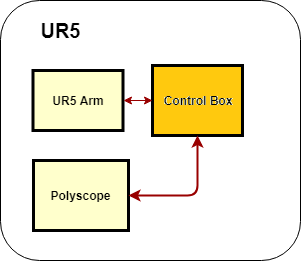
\includegraphics[width=0.60\textwidth]{images/UR5_Layer_Control_Box}
 \caption{UR5 Control Box subsystem diagram}
\end{figure}

\subsubsection{Control Box Arm Subsystem Hardware}
It contains servos various computing equipment (motherboard, hard drive, etc.)

\subsubsection{Control Box Subsystem Operating System}
This subsystem runs Linux.

\subsubsection{Control Box Subsystem Software Dependencies}
A Java Runtime Environment of at least 6.0 is required to run the UI displayed on the Polyscope.

\subsubsection{Control Box Subsystem Programming Languages}
N/A

\subsubsection{Control Box Subsystem Data Structures}
N/A

\subsubsection{Control Box Subsystem Data Processing}
N/A

\subsection{Polyscope}
A large touch pad that serves as the main UI for a user when developing for the UR5.

\begin{figure}[h!]
	\centering
 	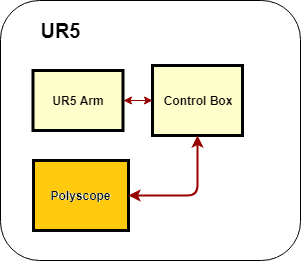
\includegraphics[width=0.60\textwidth]{images/UR5_Layer_Polyscope}
 \caption{UR5 Control Box subsystem diagram}
\end{figure}

\subsubsection{Polyscope Subsystem Hardware}
It contains a touch sensitive screen as well as a cable made solely for connecting to the UR5's control box. A emergency stop button is also located on the pad for safety reasons.

\subsubsection{Polyscope Subsystem Operating System}
N/A

\subsubsection{Polyscope Subsystem Software Dependencies}
N/A

\subsubsection{Polyscope Subsystem Programming Languages}
N/A

\subsubsection{Polyscope Subsystem Data Structures}
N/A

\subsubsection{Polyscope Subsystem Data Processing}
N/A